%05/02 - Raúl Guantes
\chapter{Sistemas dinámicos no lineales}
\section{Crecimiento logístico}
El crecimiento de las poblaciones biológicas está limitado por la disponibilidad de recursos. Para modelar este fenómeno, se introduce un nuevo parámetro $k$, que representa la capacidad de carga del entorno, es decir, la cantidad máxima de individuos que el entorno puede sostener (la cantidad de recursos disponibles para toda la población). Además, se considera:
\begin{itemize}
\item $r$: la \textbf{tasa de crecimiento} de una población (positiva)
\item $N(t)$: el número de células en el tiempo $t$
\end{itemize}
La dinámica de la población se describe mediante una ecuación diferencial que depende de $N$, $r$ y $k$:
$$\frac{dN}{dt} = f(N; r, k)$$

\subsection{Ecuación de crecimiento logístico}
Si los recursos son ilimitados, la población crece exponencialmente:
$$\frac{dN}{dt} = rN$$

Sin embargo, cuando los recursos son limitados, el crecimiento se ve afectado por la disponibilidad de recursos. Si la población supera la capacidad de carga ($N > k$), la población disminuye debido a la falta de recursos. Por el contrario, si la población es pequeña ($N < k$), hay suficientes recursos para que la población crezca. Esto se modela mediante la \textbf{ecuación de crecimiento logístico}:
$$\frac{dN}{dt} = rN(1-\frac{N}{k})$$
Esta ecuación es \textbf{no lineal} debido al término $N^2$. Se puede obtener la derivada para ver si la población crece (derivada positiva) o disminuye (derivada negativa).

\subsection{Solución de la ecuación logística}
La solución analítica de la ecuación logística es:
$$N(t) = \frac{N(0) k}{N(0) + (k - N(0))e^{-rt}}$$
Cuando $t \rightarrow \infty$, la población tiende a la capacidad de carga $k$, alcanzando un \textbf{estado de equilibrio}:
$N(t) \rightarrow k$

\subsection{Puntos de equilibrio y estabilidad}
En un sistema dinámico, los \textbf{puntos de equilibrio} son aquellos en los que la derivada temporal es cero ($dN/dt = 0$). Para la ecuación logística, los puntos de equilibrio son:
$$0 = r N (1 - \frac{N}{K}) \begin{cases} 
N^1_{eq} = K \rightarrow \text{Estable} \\
N^2_{eq} = 0 \rightarrow \text{Inestable}
\end{cases}
$$

\begin{itemize}
\item $N_{eq} = k$ es un punto de equilibrio estable, ya que la población tiende a $k$ a largo plazo.
\item $N_{eq} = 0$ es un punto de equilibrio inestable, ya que cualquier pequeña perturbación hará que la población crezca hacia $k$.
\end{itemize}

\begin{figure}[h]
\centering
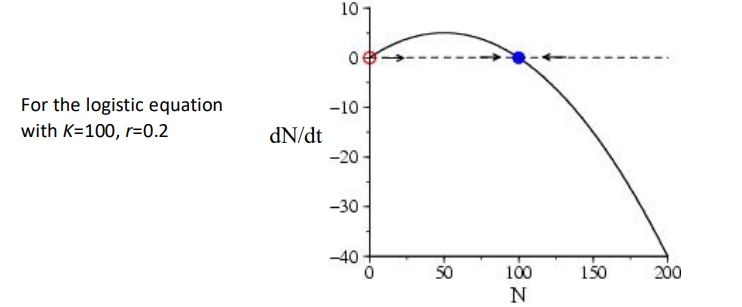
\includegraphics[width = 0.9\textwidth]{figs/estabilidad-dinamica.png}
\end{figure}

\subsection{Análisis de estabilidad}
Para entender el comportamiento a largo plazo de un sistema dinámico, es necesario calcular los puntos de equilibrio y determinar su estabilidad. 
Un sistema biológico de verdad, al medir a tiempos largos, siempre va a estar en un estado de equilibrio estable, al ser robustos a fluctuaciones. La estabilidad se puede deducir sin resolver la ecuación diferencial mediante dos formas: la forma gráfica y la forma matemática. 

\subsubsection{Método gráfico: Plano de fases}
En sistemas con una sola variable, se utiliza el plano de fases, donde:
\begin{itemize}
\item El eje x representa la variable $N$.
\item El eje y representa la derivada $dN/dt$
\end{itemize}
Para la ecuación logística:
$$\frac{dN}{dt} = f(N) = rN - \frac{rN^2}{K}$$ 
Esta función es una parábola invertida con puntos de corte en $N = 0$ y $N = k$. El máximo de la parábola se encuentra en:
$$\frac{df}{dN} = 0 \rightarrow r - \frac{2rN}{k} = 0 \rightarrow N = \frac{k}{2}$$

El punto $N = k$ es \textbf{estable} porque, a su izquierda, $dN/dt > 0$ (la población crece), y a su derecha, $dN/dt < 0$ (la población decrece).

\subsubsection{Método matemático: Linealización}
Este método es más general y puede aplicarse a sistemas con múltiples variables. Consiste en linealizar la función $f(N)$ alrededor de un punto de equilibrio $N_{eq}$ utilizando una \textbf{aproximación de Taylor}.
\begin{enumerate}
\item \textbf{Perturbación alrededor del equilibrio}
$$N = N_{eq} + \Delta N$$

\item \textbf{Derivada temporal}
$$\frac{dN}{dt} = \frac{d(N_{eq} + \Delta N)}{dt} = f(N_{eq} + \Delta N)$$

\item \textbf{Aproximación de Taylor} $f(N) \approx a + bN + cN^2 + dN^3 + \ldots$
$$f(N_{eq} + \Delta N) \approx f(N_{eq}) + \frac{df(N_{eq})}{dN} \Delta N$$
Como $f(N_{eq}) = 0$ (punto de equilibrio), se simplifica a:
$$\frac{d \Delta N}{dt} \approx f'(N_{eq}) \Delta N$$

\item \textbf{Solución de la ecuación linealizada}
$$\Delta N(t) = \Delta N(0) \cdot e^{f'(N_{eq})t}$$
\begin{itemize}
\item Si $f'(N_{eq}) > 0$, el punto de equilibrio es \textbf{inestable}, ya que la perturbación crece con el tiempo.
\item Si $f'(N_{eq}) < 0$, el punto de equilibrio es \textbf{estable}, ya que la perturbación decrece con el tiempo.
\item Si $f'(N_{eq}) = 0$, entonces se necesitan incluir términos de mayor orden de la serie de Taylor. 
\end{itemize}
\end{enumerate}

%13/02 - Raúl Guantes
\section{No linealidades superiores: biestabilidad y efecto Allee}
Si las células cooperan, el crecimiento de la población depende de su tamaño: existe un umbral en el tamaño de la población, $N*$, por debajo del cual la población se extingue. 

Para que la población crezca, no solo es necesario que tenga los recursos en el medio, si no que coopere, es decir, que haya un tamaño mínimo para que la cooperación sea efectiva. Si $N < N*$, no hay cooperación y la población disminuye, es decir, la derivada es negativa. Si $N > N*$, sí hay cooperación y N aumenta en el tiempo (la derivada es positiva).
$$\frac{dN}{dt} = rN (1 - \frac{N}{k}) (\frac{N}{N*} - 1)$$

A continuación calculamos los puntos de equilibrio y vemos su estabilidad de forma gráfica:
\begin{itemize}
\item $N^1_{eq} = 0$: estable
\item $N^2_{eq} = N*$: inestable
\item $N^3_{eq} = K$: estable
\end{itemize}

\begin{figure}[h]
\centering
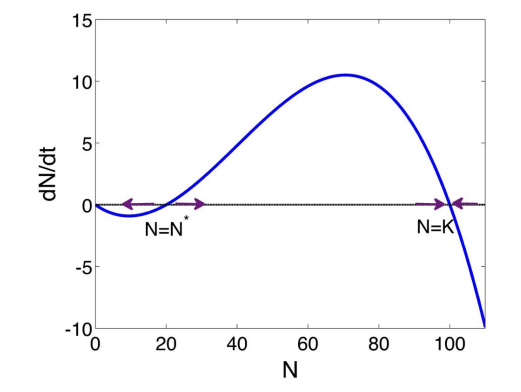
\includegraphics[width = 0.7\textwidth]{figs/bistability-graph.png}
\end{figure}

La coexistencia de dos estados de equilibrio estables se denomina \textbf{biestabilidad} (multiestabilidad para múltiples estados de equilibrio estables). Para saber a cuál va a tender la población, depende de las condiciones iniciales. Para un valor mayor de $N*$, la población tenderá a k; para un valor menor, tenderá a 0. De forma gráfica, el estado de equilibrio inestable va a servir como separador de aquellos estados de equilibrio estables. 

\begin{figure}[h]
\centering
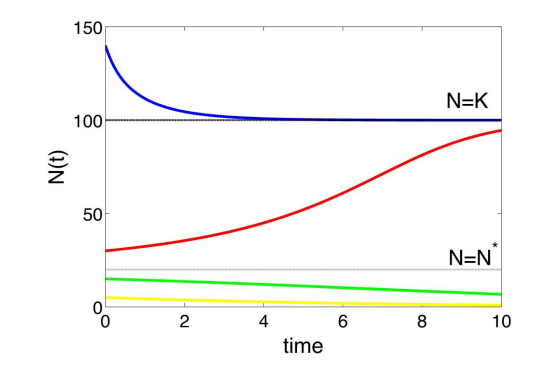
\includegraphics[width = 0.7\textwidth]{figs/bistability.png}
\end{figure}

Al cambiar el valor de los parámetros como $N*$, aparecen bifurcaciones: pueden aparecer o desaparecer puntos de equilibrio, o estos pueden cambiar su estabilidad. La bifurcación siempre ocurre a un valor determinado de los parámetros

\begin{figure}[h]
\centering
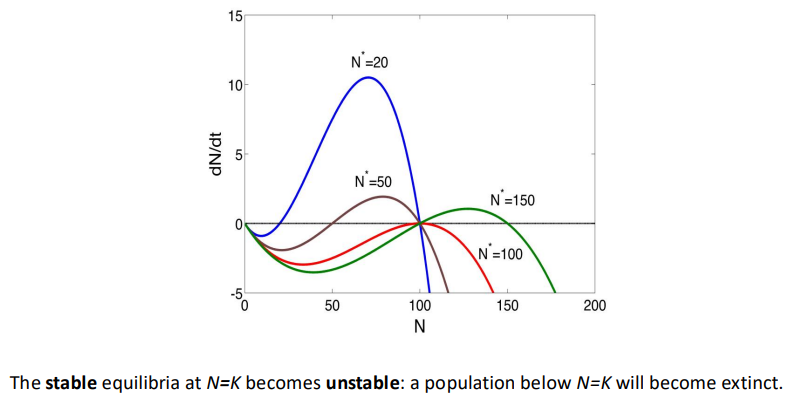
\includegraphics[width = 0.7\textwidth]{figs/bistability-bifurcations.png}
\caption{K está fijado, y N* se va aumentando progresivamente, independientemente de su sentido biológico. La línea roja representa un valor N*=k, y a partir de ahí cambia la estabilidad; ese es el punto de bifurcación, y en ese punto la derivada es 0 y la linealización falla.}
\end{figure}

Una forma cómoda de visualizar la estructura de los puntos de equilibrio y la bifurcación es trazar un diagrama de bifurcación: trazar los distintos equilibrios en función de un parámetro.

\begin{figure}[h]
\centering
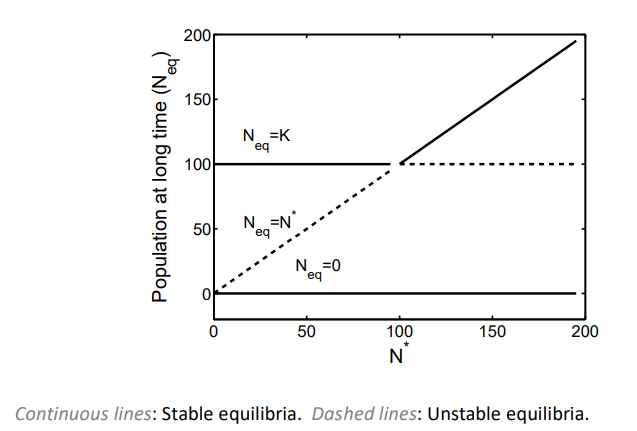
\includegraphics[width = 0.7\textwidth]{figs/bifurcation-diagram.png}
\caption{Diagrama de bifurcación. Las líneas continuas representan los estados estables, y las líneas discontinuas los estados inestables. Se representan los tres puntos de equilibrio 0, k y N*. El punto (0,0) se considera punto de bifurcación, ya que es donde cambian de estabilidad los puntos de equilibrio k y N*.}
\end{figure}

\subsection{Muerte por macrófacos: biestabilidad con histéresis}
Suponemos que tenemos una población de células inmunes (macrófagos) fija que mata células cancerígenas. La población de células cancerígenas cambia en el tiempo con la siguiente función:
$$\frac{dN}{dt} = rN(1 - \frac{N}{K}) - p(N)$$
siendo $p(N)$ el efecto de los depredadores sobre las presas: $p(N) = \frac{N^2}{1 + N^2}$
$$\frac{dN}{dt} = rN(1 - \frac{N}{K}) - \frac{N^2}{1 + N^2}$$

Para obtener los puntos de equilibrio:
$$rN (1 - \frac{N}{k} = \frac{N^2}{1 + N^2} \rightarrow r(1 - \frac{N}{k}) = \frac{N}{1 + N^2}$$
El primer punto de equilibrio es en 0. Para el resto, se pueden solapar las rectas $r(1 - \frac{N}{k})$ sobre la función $\frac{N}{1 + N^2}$ y ver los puntos de corte. Dependiendo de r, puede haber de 1 a 4 puntos de corte. 

\begin{figure}[h]
\centering
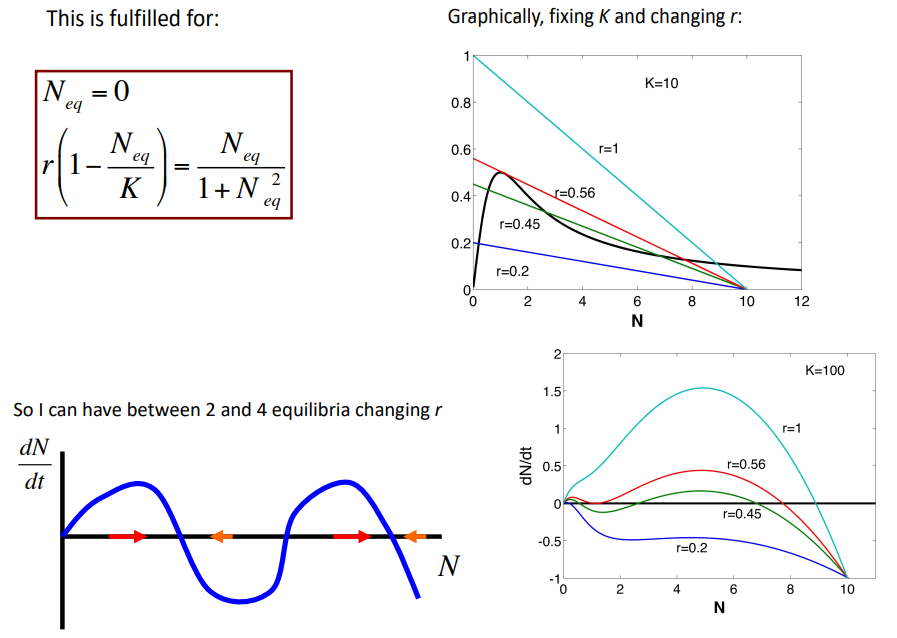
\includegraphics[width = 0.7\textwidth]{figs/biestabilidad-histeresis.png}
\caption{El estado 0 es trivial, es inestable. Si hay varios puntos de equilibrio estables, entre ellos siempre debe haber un estado inestable.}
\end{figure}

Si dibujamos este diagrama de bifurcación, hay un punto en el cuál se diferencian los puntos estable e inestable. Hay dos bifurcaciones: una donde se generan dos puntos de equilibrio y otra en el que desaparecen.

\begin{figure}[h]
\centering
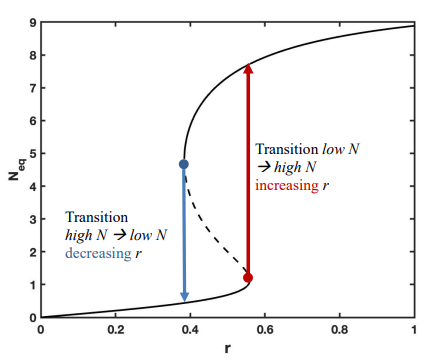
\includegraphics[width = 0.7\textwidth]{figs/bifurcation-diagram-log.png}
\caption{Diagrama de bifurcación. Para el sistema se fija k y se va alterando r. }
\end{figure}

Si incrementamos r, llegará un valor en que se da un salto brusco. Si se hace el mismo experimento disminuyendo r, la transición brusca se da a un valor distinto que en el caso anterior. A esto se le conoce como \textbf{histéresis.} El comportamiento del sistema no es simétrico. 

\section{Posibles bifurcaciones en sistemas dinámicos con 1 variable}
Esta teoría demuestra que cada bifurcación posible se puede representar por un modelo mínimo, un polinomio sencillo. Cada bifurcación es un polinomio sencillo denominado como formas normales.

La función normal $r + x^2$ recibe el nombre de \textbf{silla nodo}. Cuando cambia el parámetro $r$, hay dos puntos de equilibrio en $\pm \sqrt{-r}$. El que tenga signo negativo sería el punto estable, y el del signo positivo inestable. Si r es positivo, no hay punto de equilibrio (no se puede hacer una raíz cuadrada de un valor negativo). Por tanto, solo hay puntos de equilibrio cuando r es negativo. Para $r = 0$, tenemos el punto de bifurcación. 

\begin{figure}[h]
\centering
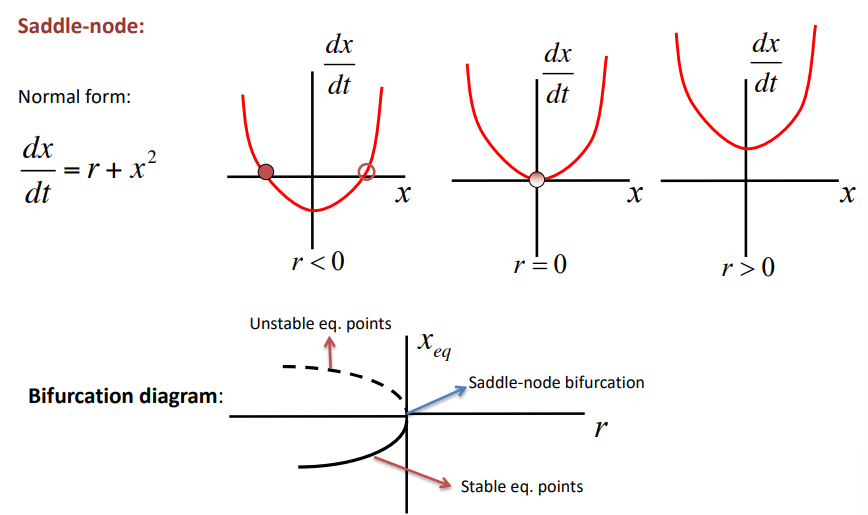
\includegraphics[width = 0.7\textwidth]{figs/saddle-node.png}
\end{figure}

Hay otras dos bifurcaciones con una sola variable: la bifurcación transcrítica y la bifurcación tridente.
\begin{figure}[h]
\centering
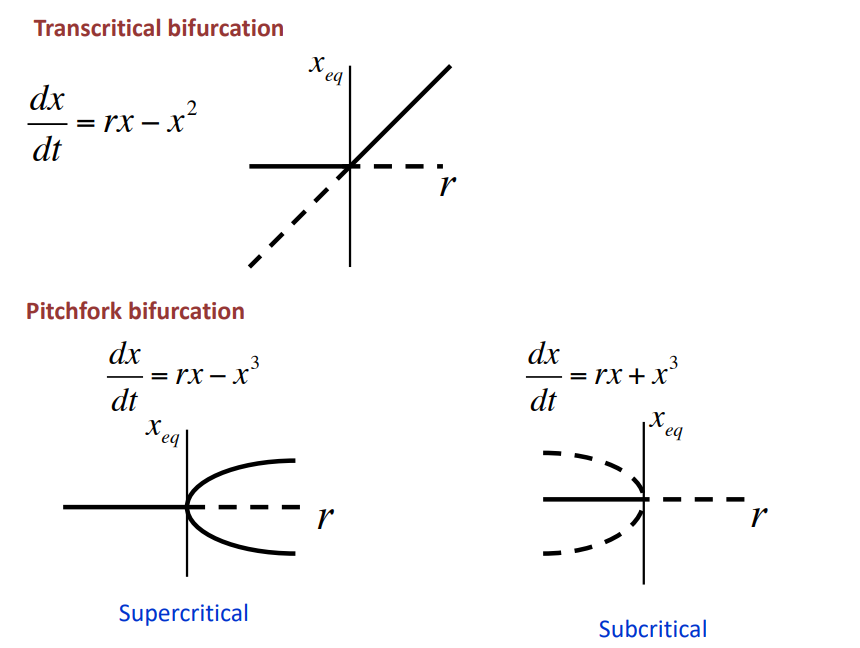
\includegraphics[width = 0.7\textwidth]{figs/bifurcacion-normal.png}
\end{figure}

La estabilidad total (número de estados posibles estables e inestables) antes y después de la bifurcación se conserva. 

\section{Sistemas dinámicos no lineales con dos variables}
\subsection{Modelo de Lotka-Volterra}
Consideremos otros tipos de interacciones entre el tumor y las células asesinas: cuando las células asesinas (células del sistema inmunitario) entran en contacto con las células tumorales, liberan señales que hacen que el organismo cree más células inmunitarias. 

La población de células asesinas depende de la población de células tumorales: ecosistema presa-predador. Ahora tenemos dos variables: $N$ son las presas, el número de células cancerígenas, y $P$ los predadores, el número de células inmunes. 
\begin{align*}
\frac{dN}{dt} = N(a - bP) && \frac{dP}{dt} = P(cN - d)
\end{align*}
A este modelo también se le conoce como \textbf{modelo Lotka-Volterra}. 

En este modelo tenemos 4 parámetros: crecimiento de presas (a), muerte de presas (b), crecimiento predadores (c), muerte predadores (d). Eso es un modelo complejo, y se puede simplificar cambiando variables "adimensionales". Siendo $u = cN/d$, $v = bP/a$ y $\tau = at$, podemos definir:
\begin{align*}
\frac{du}{d\tau} = u(1 - v) && \frac{dv}{d\tau} = \alpha v(u - 1)
\end{align*}

Ahora, los puntos de equilibrio solo dependen de $\alpha$ y se componen por dos valores:
$$\begin{pmatrix}
\frac{du}{d\tau}, \frac{dv}{d\tau}
\end{pmatrix} = (0,0) \begin{cases}
(u_{eq}, v_{eq}) = (0,0) \\
(u_{eq}, v_{eq}) = (1,1) 
\end{cases}$$

Para calcular la estabilidad, se pueden pintar por separado las ecuaciones. En el plano de variables u v, se pueden pintar por separado e igualar a cero. Así, se obtienen las nulclinas, y hay dos: la nulclina de u que hace la derivada temporal de u y la nulclina de v, que es la derivada temporal de v. Las nulclinas u y v son rectas en 1. Las dos nulclinas se cortan en el punto de equilibrio, siendo así (1,1).

\begin{figure}[h]
\centering
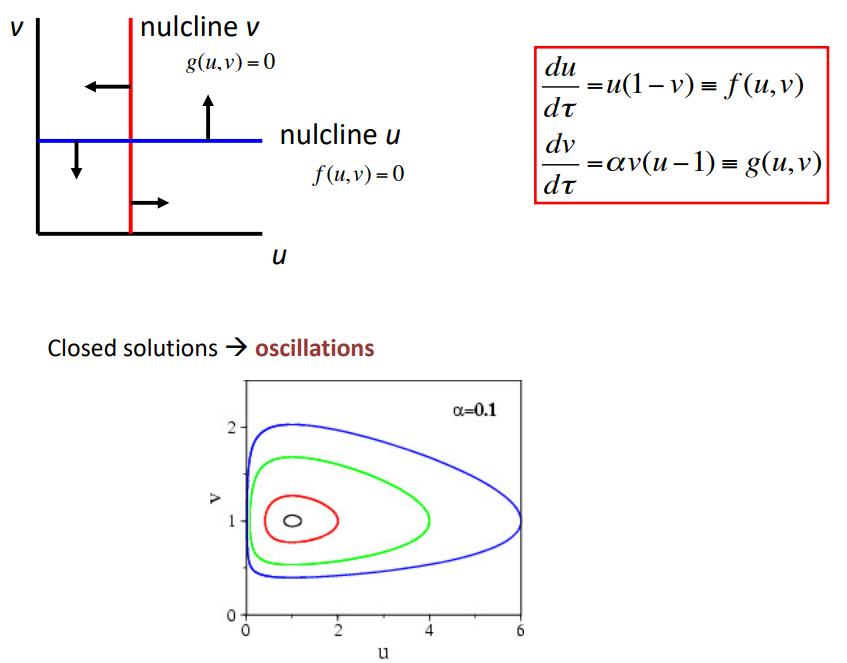
\includegraphics[width = 0.8\textwidth]{figs/nulclinas.png}
\end{figure}

El flujo va en dos direcciones al estar compuestos por un valor de u y otro de v. En una nulclina, el flujo solo va a ser en una dirección, vertical u horizontal. En la nulclina u, el flujo va a ser vertical (en la v) en la dirección según el signo de la derivada; si $u > 1$, el signo de la derivada es positivo y, por tanto, el movimiento es vertical hacia arriba, mientras que si $u < 1$, la derivada es negativa y el movimiento es vertical hacia abajo. 

El punto de equilibrio (1,1) tiene oscilaciones a su alrededor; sigue un comportamiento periódico. Las oscilaciones dependen de la condición inicial. La amplitud y el periodo van cambiando en función de lo lejos que estén del punto de equilibrio. Esto se conoce en física como un \textbf{sistema conservativo}.
Si para un mismo parámetro $\alpha$ cambiamos las condiciones iniciales, las oscilaciones van a cambiar. Las oscilaciones biológicas suelen ser robustas (no cambian de periodo ni de amplitud) con respecto a las condiciones y parámetros iniciales, solo en función de los parámetros.